% -*- TeX:UK -*-
\documentclass[10pt]{beamer}
\usetheme{metropolis}
%\useinnertheme{rectangles}
\setbeamercovered{%
still covered={\opaqueness<1->{15}},
again covered={\opaqueness<1->{40}}}

\hypersetup{colorlinks,linkcolor=black,urlcolor=brown,citecolor=brown}

\usepackage{amsmath,amssymb,amsthm}
\usepackage{unicode-math}

% We set the Lucida OTF fonts as default
\usepackage{fontspec}
\setmainfont{Lucida Bright OT}
\setsansfont{Lucida Sans OT}
\setmonofont{Lucida Console DK}[Scale=MatchLowercase]

\newfontfamily\webglyphsfont{WebHostingHub-Glyphs}[Scale=0.7]
\newcommand\webglyphs[1]{{\webglyphsfont\symbol{#1}}}
\newcommand\Discussion{\colorbox{white}{\textcolor{black}{\webglyphs{"F134}}}\xspace}
\newcommand\DiscussionI{\colorbox{black}{\textcolor{white}{\webglyphs{"F134}}}\xspace}
\newcommand\DExamples{\colorbox{black}{\textcolor{white}{\webglyphs{"F134} examples?}}}
\newcommand\Reading{\colorbox{black}{\textcolor{white}{\webglyphs{"F0C1}}}\xspace}
\newcommand\ReadingI{\colorbox{white}{\textcolor{black}{\webglyphs{"F0C1}}}\xspace}
\newcommand\Video{\colorbox{white}{\textcolor{black}{\webglyphs{"F03D}}}\xspace}
\newcommand\Attention{\colorbox{black}{\textcolor{orange}{\webglyphs{"F05A}}}\xspace}
\newcommand\HomeWork{\colorbox{white}{\textcolor{black}{\webglyphs{"F5ED}}}\xspace}
\newcommand\HomeWorkI{\colorbox{black}{\textcolor{white}{\webglyphs{"F5ED}}}\xspace}
\newcommand\Advanced{\colorbox{black}{\textcolor{white}{\webglyphs{"F235}}}\xspace}

\newfontfamily\lineabasicfont{linea-basic-10}
\newcommand\basicicons[1]{{\lineabasicfont\symbol{#1}}}
\newcommand\timeforwards{\basicicons{"0079}}
\newcommand\timebackwards{\basicicons{"0064}}

\newfontfamily\lineaweatherfont{linea-weather-10}
\newcommand\weathericons[1]{{\lineaweatherfont\symbol{#1}}}
\newcommand\meteosun{\weathericons{"E038}}
\newcommand\meteosuncloud{\weathericons{"E042}}
\newcommand\meteorain{\weathericons{"E033}}
\newcommand\meteowind{\weathericons{"E054}}

\newfontfamily\uleaffont{Mini Pics Uprooted Leaf}
\newcommand\uleafmpics[1]{{\uleaffont\symbol{#1}}}
\newcommand\lowplants{\uleafmpics{"00CE}}
\newcommand\mediumplant{\uleafmpics{"006A}}
\newcommand\bush{\uleafmpics{"0039}}
\newcommand\smallplant{\uleafmpics{"0030}}
\newcommand\seedling{\uleafmpics{"002F}}
\newcommand\floweringplant{\uleafmpics{"00CA}}

\newfontfamily\utwigfont{Mini Pics Uprooted Twig}
\newcommand\utwigmpics[1]{{\utwigfont\symbol{#1}}}
\newcommand\grassplant{\utwigmpics{"0033}}

\newfontfamily\uinsectfont{Insect Icons}
\newcommand\uinsect[1]{{\uinsectfont\symbol{#1}}}
\newcommand\bug{\uinsect{"006F}}

\usepackage{polyglossia}
\setdefaultlanguage[variant = british, ordinalmonthday = false]{english}

\usepackage[style=authoryear-comp,firstinits,sortcites,maxcitenames=2,%
    mincitenames=1,maxbibnames=10,minbibnames=10,uniquename=mininit,%
    uniquelist=minyear,sortfirstinits=true]{biblatex}
\addbibresource{../references/ecophys.bib}
\renewcommand{\bibfont}{\small}

\usepackage{abbrev}



\begin{document}

\title{PBIO-141\\Sensory and Physiological Ecology\\ of  Plants}
\subtitle{3: Signals, cues, information and evolution}
\author{Pedro J. Aphalo}
\date{January--February 2022}
\institute[Univ.\ of Helsinki]{M.Sc.\ in Plant Biology, University of Helsinki\\[2ex] \url{http://blogs.helsinki.fi/aphalo/}}

  \begin{frame}
    \maketitle
  \end{frame}

  \begin{frame}[c]
    \begin{center}
      \begin{small}
        \copyright 2006--2022 by Pedro J. Aphalo\\
        University of Helsinki, Finland.\\
        \textcolor{blue}{\url{http://blogs.helsinki.fi/senpep-blog/}}\\[2ex]
      \end{small}

      \begin{footnotesize}
        Sensory and Physiological Ecology of Plants slides by Pedro J. Aphalo are licensed under a Creative Commons Attribution-ShareAlike 4.0 International License.

      
\includegraphics[width=6em]{../figures/copyright/by-sa}\\[2ex]
      \end{footnotesize}
        
        \begin{scriptsize}
        Typeset in Lucida Sans, \textrm{Luicda Bright}, \texttt{Lucida Console} and Lucida Math. Icons from fonts ``WebHostingHub Glyphs'' (under SIL-Open Font License) from \url{https://www.webhostinghub.com/}; ``insect icons'' (free from \url{http://www.woodcutter.es/}); ``linea-basic-10'' and ``linea-weather-10'' (free from \url{https://github.com/linea-io}), ``Mini Pics Uprooted Twig'' and ``Mini Pics Uprooted Twig'' (commercial, from Image Club Graphics, Inc.). Plant icon as .svg by Abdul Wahhab (free from \url{NounProject.com}).

        Illustrations and text quoted from copyrighted sources is excluded from this license and their use should respect the original licenses.
        \end{scriptsize}
    \end{center}
  \end{frame}


  \begin{frame}
    \frametitle{Outline}
    \tableofcontents
  \end{frame}

\section{Hierarchy and scale}
\nocite{Allen1982}

\begin{frame}{Levels of organization}
An example of a hierarchy is the hierarchy of levels of organization

Ecosystem $\rightarrow$\\
\hspace{.5cm}Community $\rightarrow$\\
\hspace{1cm}Population $\rightarrow$\\
\hspace{1.5cm}Individual $\rightarrow$\\
\hspace{2cm}Organ $\rightarrow$\\
\hspace{2.5cm}Tissue $\rightarrow$\\
\hspace{3cm}Cell $\rightarrow$\\
\hspace{3.5cm}Organelle $\rightarrow$\\
\hspace{4cm}Molecule $\rightarrow$\\
\hspace{4.5cm}Atom $\rightarrow$\\
\hspace{5cm}Subatomic particle

\end{frame}

\begin{frame}{Scale}
    \begin{description}[type=1]
        \item[Temporal scale] Fast physiological
        responses, acclimation, and adaptation happen at
        different temporal scales. The processes involved are
        different.
        \item[Spatial scale] For example when
        studying transpiration, we can do it at different
        scales: the leaf, the tree crown, the forest, etc.
        The main controlling environmental variables may
        be different.
    \end{description}
\end{frame}

\begin{frame}{Mechanism and `reason' (=justification)}
    \begin{itemize}
        \item \emph{Upward and downward causation} in biology.
        \item We achieve a \emph{mechanistic explanation} for an
        observed phenomenon by studying the levels below.
        e.g. We study whole plant growth in two different habitats.
        We build a mechanistic
        explanation from the growth and responses of individual
        organs: leaves, stems, roots.

        \item We build a \emph{narrative explanation} for the phenomenon
        by looking at the levels above.
        e.g. In this example we find a reason or justification for
        the differences based on natural selection, but we do not study
        the evolutionary process itself.

        \item Of course we can set the focus at any level in the hierarchy and what is mechanism or narrative explanation will move along.~\DExamples
    \end{itemize}
\end{frame}

\begin{frame}{Cause and effect in Biology \Discussion 10 + 5 min}

\begin{centering}
$\to$ \emph{fitness} $\to$ genome $\to$  epigenome $\to$ phenome $\to$ \emph{fitness} $\to \cdots$
\vspace{3ex}
\end{centering}

\begin{description}
%  \item[time sequence] .
  \item[\DiscussionI] Which transitions, shown as $\to$, depend directly on the environment?
  \item[\DiscussionI] ``Evolution determines physiology'' or ``Physiology determines fitness''?
  \item[\Attention] The course of evolution is not the result of natural selection alone!
\end{description}
\pause
\Attention \emph{Multiple viewpoints are possible, and not necessarily contradictory!}
\end{frame}

\section{Controversies in plant sensory biology}

\begin{frame}
\frametitle{Recent controversial concepts in plant biology}
\begin{itemize}
\item Plant communication $\rightarrow$ \textcolor{green}{Widely accepted}
\item Plant behaviour $\rightarrow$ \textcolor{yellow}{Mild controversy}
\item Plant intelligence $\rightarrow$ \textcolor{orange}{Strong controversy}
\item Plant consciousness $\rightarrow$ \textcolor{orange}{Widely rejected}
\item Plant neurobiology $\rightarrow$ \textcolor{red}{Widely rejected}
\end{itemize}
\end{frame}

\begin{frame}
\frametitle{A problem of terminology}
\begin{itemize}
\item Plant communication $\rightarrow$ \textcolor{green}{meaning is clear}
\item Plant behaviour $\rightarrow$ \textcolor{yellow}{meaning is fuzzy}
\item Plant intelligence $\rightarrow$ \textcolor{orange}{meaning is obscure}
\item Plant consciousness $\rightarrow$ \textcolor{orange}{meaning is opaque}
\item Plant neurobiology $\rightarrow$ \textcolor{red}{meaning is contradictory}
\end{itemize}
\end{frame}

\begin{frame}
\frametitle{A problem of experimental evidence}
\begin{itemize}
\item Plant communication $\rightarrow$ \textcolor{green}{strong evidence}
\item Plant behaviour $\rightarrow$ \textcolor{green}{strong evidence}
\item Plant intelligence $\rightarrow$ \textcolor{yellow}{depends on definition}
\item Plant consciousness $\rightarrow$ \textcolor{red}{known unknowable (?)}
\item Plant neurobiology $\rightarrow$ \textcolor{red}{no evidence of function}
\end{itemize}
\end{frame}

\begin{frame}{Some publications}
  \citetitle{Aphalo1995} \cite{Aphalo1995}\\
  \citetitle{Trewavas2014} \cite{Trewavas2014}\\
  \citetitle{Taiz2019} \cite{Taiz2019}\\
  \citetitle{Aphalo2021a} \cite{Aphalo2021a}
\end{frame}

\section{A different controversy}

\begin{frame}
\frametitle{The need for context awareness}
\begin{itemize}
\item \emph{I exclude here the controversy about GMO themselves.}
\item Genetic manipulation has worked for breeding simple traits $\rightarrow$ \textcolor{green}{no controversy}
\item Genetic manipulation has worked for complex traits $\rightarrow$ \textcolor{orange}{strong controversy}
\item To an agronomist producing a GMO crop genotype with more efficient photosynthetic metabolism is a success only if it results \emph{in a cultivar with improved performance in farms}.
\item That some molecular biologists consider/``sell'' such a result on photosynthesis as a breakthrough towards ending famine or some similar major goal can deeply upset most agronomists\ldots
\end{itemize}
\end{frame}

\begin{frame}
\frametitle{What is the evidence}
\begin{itemize}
\item Genetic manipulation has worked for breeding simple traits $\rightarrow$ \textcolor{green}{strong evidence}
\item Genetic manipulation has worked for complex traits $\rightarrow$ \textcolor{orange}{one or two isolated ``special cases'' out of very many attempts}
\item In my view the problem is not in GM as a method, it is in not understanding that improvement in a trait like photosynthesis rate is almost never directly reflected in yield
\item An organism is like a choir, if a single singer starts singing louder than others, it makes the performance of the choir worse rather than better, unless the singer is a solist\ldots
\end{itemize}
\end{frame}

\begin{frame}{Some publications}
  \citetitle{Zhu2010} \cite{Zhu2010}\\
  \citetitle{Denison2012} \cite{Denison2012}\\
  \citetitle{Evans2013} \cite{Evans2013}\\
  \citetitle{Sadras2021} \cite{Sadras2021}\\
  \citetitle{Passioura2020} \cite{Passioura2020}\\
  \citetitle{Sinclair2019} \cite{Sinclair2019}\\
\end{frame}

\section{Experiments and surveys}

\begin{frame}{Types of experiments (refresher)}
\begin{small}
    \begin{description}[type=1]
        \item[Manipulative experiments.] With manipulative experiments it
        is possible to \emph{directly} demonstrate cause-effect relationships.

        \item[Observational experiments.] When manipulative experiments
        are not possible, direct demonstration of cause-effect
        relationships can be very difficult.

        \item[Impossible experiments.] In many situations
        manipulative experiments are physically or ethically
        impossible to carry out.

        \item[Simulations.] When we do experiments with models
        instead of the real system we call them simulations.

        \item[\DExamples]

    \end{description}
\end{small}
\end{frame}

\begin{frame}{Experiments and causality}
\begin{itemize}
\item Demonstration of causes. In manipulative experiments we (attempt to) keep
everything equal among treatments except for the experimental
variable whose effect we want to test.

\item In observational studies we cannot be sure of which things
are different among the different situations (``treatments''), so we
can make guesses about causes, but can seldom directly demonstrate them.

\item In observational studies we can use path analysis to indirectly strengthen the evidence for causation (we add an additional dimension, usually time).

\item \DExamples

\end{itemize}
\end{frame}

\section{Practical = experiment}

\begin{frame}{Some ideas of treatments to test}
\begin{enumerate}
  \item Pulsed/fluctuating light vs continuous
  \item Light of different colours (visible ones)
  \item Light of different ``colours'' (ultraviolet)
  \item Different temperatures or air humidity
  \item Different daylengths
\end{enumerate}

\end{frame}

\begin{frame}{Some ideas of measurements}
\begin{enumerate}
  \item Water use (weighing)
  \item Temperature of leaves
  \item Growth
  \item Stomatal conductance
  \item Pigments (Dualex)
\end{enumerate}

\end{frame}

\section{A video for discussion}
\nocite{Falik2011,Falik2012,Novoplansky2021}

\begin{frame}{Talk by Ariel Novoplansky \Video}

Observation without preconceptions plus theory are important when developing new hypotheses\ldots

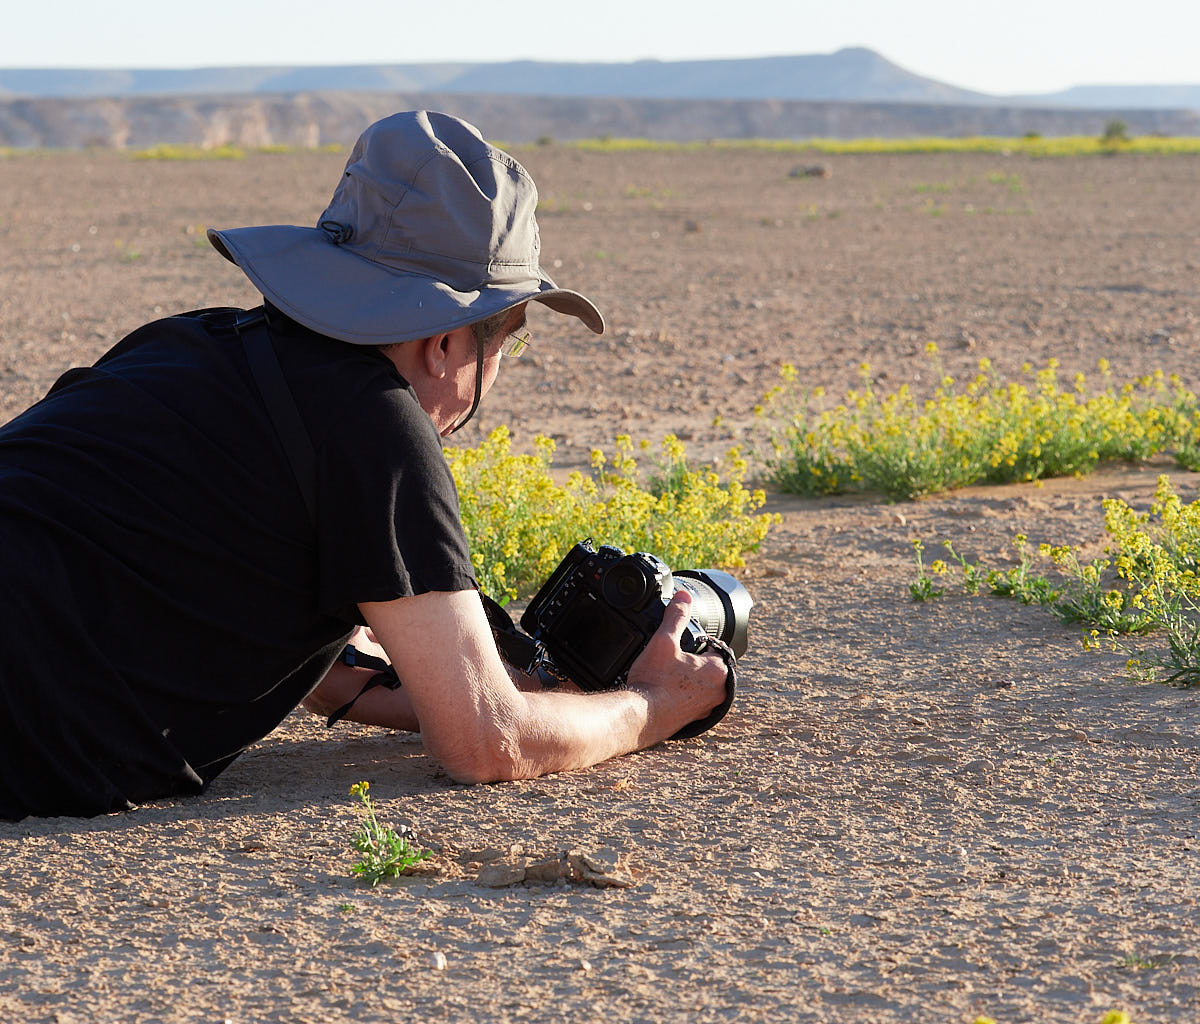
\includegraphics[width=0.5\linewidth]{photos/ariel}

 \Video (15 min) \url{https://youtu.be/aClSp71zfro}

\end{frame}


\begin{frame}{Next steps \Discussion}
\begin{itemize}
  \item By now I expect you and me to share enough of a language and frame of mind to discuss without misunderstandings.
  \item If some ideas remain unclear, do ask at any time.
  \item If we had enough time we have watched the video of the TEDx talk by Prof.\ Ariel Novoplansky, but if not please watch it at home. Discuss about it in the corresponding Moodle forum. Remember that discussion can include what implications the phenomena described may have in a question of your own interest, how watching the talk may have changed your views about plants, questions about something that you did not understand, or something that you would like to criticize.
\end{itemize}

\end{frame}



%\begin{frame}{\HomeWork Thought exercise for next class}
%
\includegraphics[width=2cm]{figures/icons-svg/noun-plant-1358991.png}
%\begin{enumerate}
%  \item Consider a plant you have at home (or another specific individual plant).
%  \item Write a list of the factors in its environment that vary through the day.
%  \item Consider the environment of roots, leaves and stems of this plant.
%  \item Consider what properties of these factors are most and least important to the growth of your plant.
%\end{enumerate}
%\end{frame}
%

  \section*{References}
  \begin{frame}[t,allowframebreaks]
    \frametitle{References}
    \printbibliography
  \end{frame}

\end{document}
